\chapter{Methodology}%
\label{chapter:methodology}

\begin{introduction}
A short description of the chapter.

A memorable quote can also be used. asas
\end{introduction} 


\section{Arquitecture}

The architecture of the application will have a \ac{MVC} pattern. 
The \ac{MVC} pattern is a software design pattern that separates the application into three main components: Model, View, and Controller.[25] [26]
The Model is responsable for the storage of data and the logic of the application.  [25] [26]
It provides an abstraction layer of the database that allows data operation without the direct contact from the user interface. [26]
It also controls the business logic of the application, such as calculations, data validation and data manipulation. [26]

The View represents the \ac{UI} of the application and is used to present the information from the Model component. [25] [26]
This component is also responsable for the user's interactions and it does not contain any logic of the application, only limits itself to the communication between the Controller and the user. [26]

The Controller acts as an intermediary between the Model and View.
It receives the user's input and it is responsable to process the data and update the Model based on the user's actions and update the view to give feedback of the changes maded. [25] [26]

This pattern is popular for designing designing applications because it provides a clean separation of concerns. This separation, increases the maintainability and reusability of the code, facilitates the creation of the test and turns the application more scalable. [25] [26]
The \ac{MVC} pattern is a popular pattern for designing applications because it provides a clean separation of concerns, making it easier to maintain and test the application. [25] [26]
This requirements are advantageous, since the functional requirements of the project are not fully stablished and may receive some suggestion from the company along the way. 
The scalability is also important since the aim market of this application are the company's dealerships that may be scattered across the country or even Europe.

The framework the application will be built with is the Asp Net Core MVC. 
I believe this approach will be better than following the successful application from the authors ... from the paper [....] for multiple reasons.
The integration with the microsoft framework MYSQL database is more simple when using ASP.NET Core due to the package Entity Framework [https://learn.microsoft.com/en-us/aspnet/entity-framework]. 
Laravel also supports this database interaction, but Asp Net Core MVC is more suitable for this environment. [18]
Additionally, Laravel loses in performance with the Compiled Language ASP.NET since it is a Interpreted language. 
In security, larabel offers some security features like hashing or secure input validation, but requires deeper PHP knowledge and proactive vulnerability management. 
Microsoft offers greater security tools that provides a major abstraction to this concept and allows the develop to focus on the application functionalities. [18]

Despite all of this advantages, the main reason to use this framework and pattern is to integrate with the Fleet Management System that has the same approach. 
Since i was involved in the project i am familiar with this tecnology, so, even though ASP.NET can have a greater learning curve for unfamiliar developers [18], I am not in that category.

Based on the feedback from the users in the study ... [23], where the authors refer a integration of a SMS notification system to remind customers of scheduled visits, i decided to integrate to this platform another application for the customers. 
This application functionality is to notify the user about the progress of the maintenance and get feedback for the service provided at the dealership.
It has the purpose of increasing the user satisfaction by keeping the client inform and gather information about future improvements.
This application will be built as a \ac{PWA} in ASP.NET Core mvc, for convinience purpose and simplicity.

To summarize, I will develop 2 application in this dissertation in ASP.NET Core to be integrated in the developed system at Lightmobie, one for the workers at the dealership and another for their clients.


\section{Fleet Management System}
The Fleet Management System is a platform for owners of a vehicle sharing system to manage their equipment. 
This platform shows the equipment information and interactions, alerts, statistics and user trips. 
It has a functionality to assign permissions and a role to a user, which it'll be beneficious in a use case that i will mention in the next chapter.   

\section{Aplications Use Cases}

The structure of the dealership application was based on the work of the author in the paper ... [11] and is separated into 4 key user roles: recepcionist, mecanic, warehouse operator and administrator.

The recepcionist will be responsable to interact with the client, this includes the vehicle check-in and check-out and user comunication in the case of changes in the inicial stablished price and vehicle actions. 
The Use cases of the recepcionist are:

\begin{itemize}
    \item Use Case 1.1 – Vehicle Reception
    \begin{itemize}
      \item Scenario – Client arrives at the dealership with a vehicle to be repaired.
      \item Objective – Create a new maintenance request in the system.
      \item System – The receptionist insert in the a form all the information about the initial maintenance request from the client as well as some superficial problem he can find and creates a new maintenance request with the date and budget agreed with the client. 
    \end{itemize}
    \item Use Case 1.2 – Vehicle Delivery 
    \begin{itemize}
      \item Scenario – The Recepcionist delivered the vehicle to the Client.
      \item Objective – Complete the vehicle maintenance process.
      \item System – Sends a report in a pdf format to the client with the information of the maintenance request and alters the maintenance request status in the system to concluded. 
    \end{itemize}
    \item Use Case 1.3 – Collect information about a maintenance request
    \begin{itemize}
      \item Scenario – A Client call the dealership to ask about the maintenance of his vehicle.
      \item Objective – Visualize the maintenance information.
      \item System –  The Receptionist searches a list of maintenance requests by vehicle/customer name/maintenance ID and, by clicking on the element details button, he can view the maintenance details.
    \end{itemize}
    \item Use Case 1.4 – Asking for customer permission
    \begin{itemize}
      \item Scenario – O problem in a vehicle maintenance has occurred and the inicial agreement with client may be broken.
      \item Objective – Inform the client of the problem and achieve an agreement.
      \item System – The Receptionist receives an alert that there has been a change in the initial maintenance budget for a vehicle and/or a change in the maintenance completion deadline, so he needs to contact the customer to inform him. Depending on customer feedback, the receptionist accepts the request, declines the request or terminates the maintenance.
    \end{itemize}
  \end{itemize}  
  \hfill \break


  The mecanic will be responsable to do the maintenance in the vehicle, like oil change, tire change, trade vehicle parts, etc. 
  It will previously evaluate the vehicle, to assure the inicial evaluation of the recepcionist isn't lacking, and after the maintenance is done, it will write a report of the operations done. 
  The mecanic Use cases are:

  \begin{itemize}
    \item Use Case 2.1 – View to-do list
    \begin{itemize}
      \item Scenario – The mecanic arrives at dealership and wants to see what tasks he has to do today.
      \item Objective – See the day's work organization.
      \item System – The mecanic watches a list of tasks that were assign from the administrator, as soon as he enters the system. Each task is accompany by a description, a priority, the vehicle identification, a set of actions to be performed and comments from other users. 
    \end{itemize}
    \item Use Case 2.2 – Carry out a vehicle analysis 
    \begin{itemize}
      \item Scenario – A new vehicle needs to be analyzed.
      \item Objective – Confirm the inicial analysis of the receptionist and search for additional problems.
      \item System – The mechanic enters the problems he finds in the vehicle into the system, as well as tasks that need to be done. 
    \end{itemize}
    \item Use Case 2.3 – Prepare a list of necessary parts
    \begin{itemize}
      \item Scenario – After vehicle analysis.
      \item Objective – Elaborate a request of vehicle parts for the warehouse.
      \item System – The mecanic selects the parts of the vehicle that need to be replaced and sends a request with the new parts to the warehouse.
    \end{itemize}
    \item Use Case 2.4 – Deliver damaged parts to the Warehouse
    \begin{itemize}
      \item Scenario – The mecanic goes to the warehouse to deliver the damaged parts.
      \item Objective – Register the parts as being damaged.
      \item System – The mecanic removes the damaged parts from the vehicle and change the status to damaged.
    \end{itemize}
  \item Use Case 2.5 – Collect the requested parts in the Warehouse
  \begin{itemize}
    \item Scenario – The mechanic goes to the warehouse to collect new parts for the vehicle.
    \item Objective – Collect parts to replace the damaged parts in the vehicle.
    \item System – The mecanic add the new parts to the vehicle in the system.
  \end{itemize}
\item Use Case 2.6 – Vehicle maintenance
\begin{itemize}
  \item Scenario – A new vehicle is ready for a maintenance.
  \item Objective – The mechanic will do the vehicle maintenance (oil change, tire change, vehicle wash…).
  \item System – The mechanic sees a set of tasks that he needs to do to complete the vehicle maintenance and whenever he finishes a task, he marks it as completed.
\end{itemize}
\item Use Case 2.7 – Making the repair report
\begin{itemize}
  \item Scenario – After vehicle maintenance.
  \item Objective – Conclude the maintenance of a vehicle.
  \item System – The Mechanic enters into the system all operations and tests carried out on the system as well as their results.
\end{itemize}
\end{itemize}
\hfill \break

The warehouse operator is responsable to manage the dealer's stock and ask for suplies, so i write the following use cases:

\begin{itemize}
  \item Use Case 3.1 – View the different parts that the warehouse possess
  \begin{itemize}
    \item Scenario – The warehouse worker wants to view the quantity of a certain parts that the warehouse possess.
    \item Objective – Show quantitative warehouse information.
    \item System – List of all parts and their quantities that the warehouse possess. 
  \end{itemize}
  \item Use Case 3.2 – Requesting purchasing service 
  \begin{itemize}
    \item Scenario – The warehouse worker discovers that he has an insufficient number of parts for maintenance or anticipates that this part will be missing soon.
    \item Objective – Request permission to purchase parts from the supplier.
    \item System – The Warehouse Worker will place a purchase order for parts. The system notifies the administrator via the platform and by email requesting authorization to do the purchase. 
  \end{itemize}
  \item Use Case 3.3 – Registration of new parts in the System
  \begin{itemize}
    \item Scenario – The warehouse purchased several parts from a supplier.
    \item Objective – Register new parts in the system.
    \item System – Warehouse operator adds a specific type of part to the system with its appropriate description and identification.
  \end{itemize}
\end{itemize}
\hfill \break

The last user of the application is the administrator or Workshop Manager. This user is in charge of managing the platform and the dealership. So the main use cases i encountered are:

\begin{itemize}
  \item Use Case 4.1 – Authorizing purchases
  \begin{itemize}
    \item Scenario –  The administrator received a purchase request.
    \item Objective – Authorize or reject a purchase authorization request.
    \item System – List of all purchase authorization requests, as well as their details. The administrator can change the status of this request, rejecting or authorizing. 
  \end{itemize}
  \item Use Case 4.2 – View history of maintenance performed
  \begin{itemize}
    \item Scenario – The administrator wants to gather information from recently performed maintenance.
    \item Objective – View information about a specific maintenance that occurred.
    \item System – List of all maintenance that occurred as well as its details (who carried it out, which parts were removed, the name of the customer, tests carried out and their results…). 
  \end{itemize}
  \item Use Case 4.3 – Develop statistics
  \begin{itemize}
    \item Scenario – The administrator wants to gather statistics on maintenance that was carried out in the last month.
    \item Objective – View information about maintenance over a given period of time.
    \item System – Presentation of the number of parts replaced, number of purchases, total price spent on new parts, remuneration for maintenance, average customer’s rating, etc.
  \end{itemize}
  \item Use Case 4.4 – Assign roles to employees
  \begin{itemize}
    \item Scenario – A new employee has been hired.
    \item Objective –  Assign roles to new employee.
    \item System – The administrator assigns the new employee a certain role and set of permissions.
  \end{itemize}
  \item Use Case 4.5 – Assign tasks to the employees
  \begin{itemize}
    \item Scenario – A new maintenance request has been requested.
    \item Objective – Assign and organize tasks to different employees.
    \item System – The administrator assigns the various stages of vehicle maintenance to the various workshop employees.
  \end{itemize}
\end{itemize}
\hfill \break

The client application will only be interacted by a role of users, the client.
The use cases are listed below:

\begin{itemize}
  \item Use Case 5.1 – View current maintenance status
  \begin{itemize}
    \item Scenario – The Customer wants to find information regarding the vehicle maintenance procedure.
    \item Objective – Display current maintenance status.
    \item System – The system will illustrate all the maintenance steps that the vehicle has already undergone, as well as those that remain to be completed. 
  \end{itemize}
  \item Use Case 5.2 – Notify the customer of the end of maintenance 
  \begin{itemize}
    \item Scenario – Vehicle maintenance has been completed and the customer can now collect the vehicle.
    \item Objective – Notify the user of the end of maintenance.
    \item System – The system will show a native notification on the customer's cell phone informing that the vehicle is ready to be picked up. 
  \end{itemize}
  \item Use Case 5.3 – Rating of the service provided
  \begin{itemize}
    \item Scenario – The client receives the vehicle and the receptionist completes the maintenance process.
    \item Objective – Get feedback from the client.
    \item System – The system will show a form to the client asking about service provided. The crucial points are time of the service, service quality, user interaction and price.
  \end{itemize}
\end{itemize}
\hfill \break

With all of this use cases, both application should increase the efficiency of the work at the dealership and improve client loyalty to ensure profit.

\section{Aplications Work flow}

After the development of the use cases i designed a flow chart to understand the users' interaction with the system and each other. The chart is visible in figure \ref{fig:figure2}.

\begin{figure}[h]
  \caption{Use Case Flow Chart of the Client, Recepcionist, Mecanic, Warehouse Operator and administrator.}
  \centering
  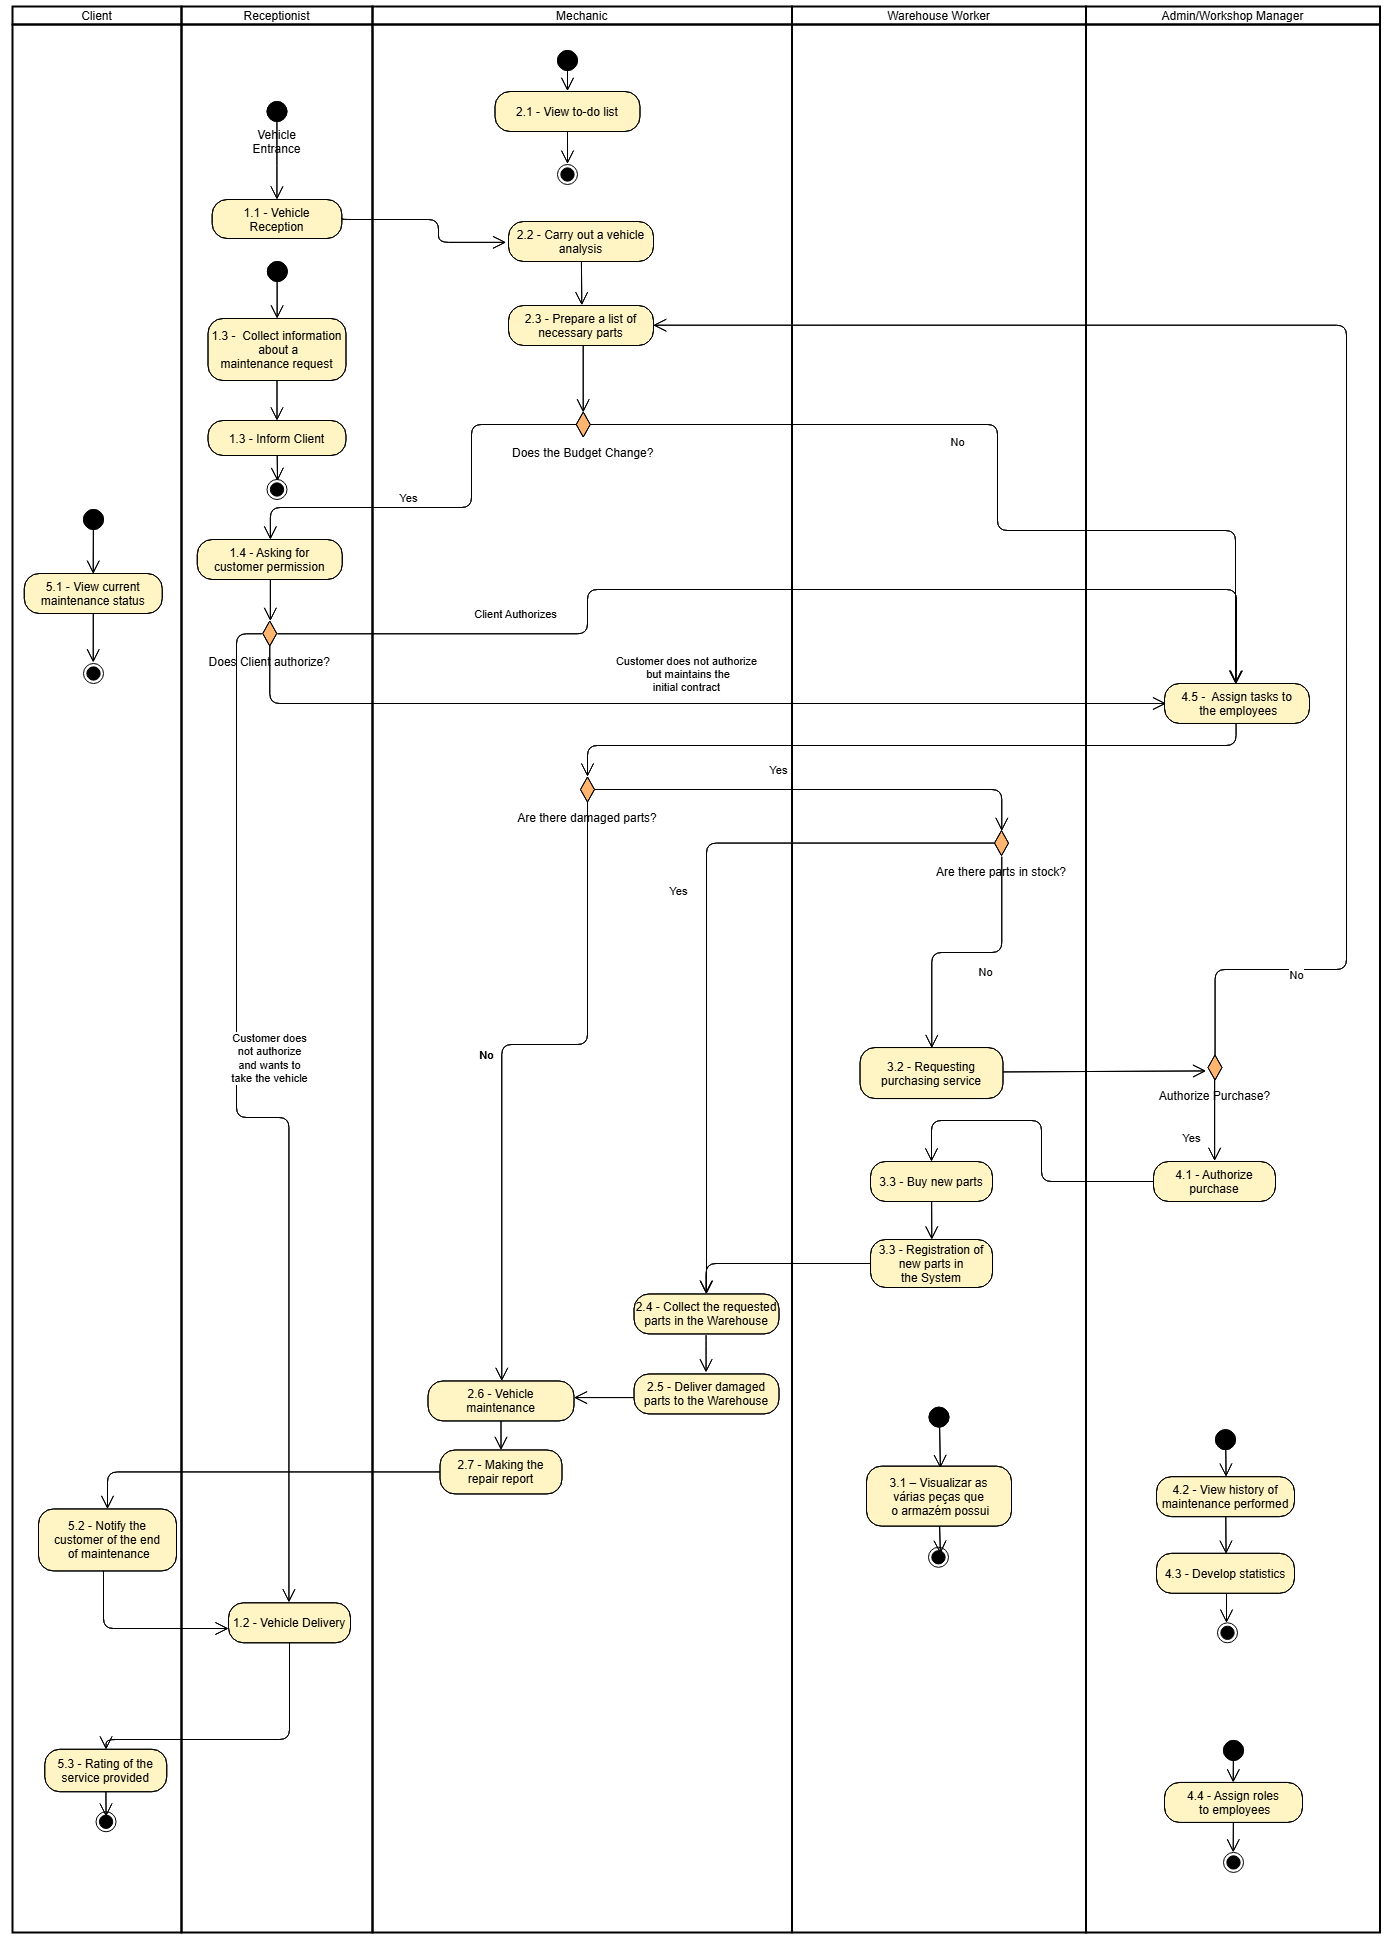
\includegraphics[width=\textwidth]{figs/UseCaseDiagram}
  \label{fig:figure2}
\end{figure}

The system main flow starts with the Use Case 1.1 when a Client arrives at the dealership for a vehicle maintenance. 
The recepcionist does a inicial a evaluation of the vehicle (if its the case) and get some inputs from the client 